\section{Model and methods}\label{sec:methods}

\subsection{Device and Lugiato--Lefever model}\label{sec:lle}

We consider a fused-silica microring resonator with a free spectral range (FSR) of $200~\mathrm{GHz}$, group index $1.45$,
ring length $L\approx1.03~\mathrm{mm}$, nonlinear coefficient $\gamma=0.016~\mathrm{W^{-1}m^{-1}}$, group-velocity dispersion
$\beta_2=-4\times10^{-27}~\mathrm{s^2/m}$ (anomalous) and a pump at $1550~\mathrm{nm}$.
The ring has an input (through) port and a drop port, and an intrinsic quality factor $\Qint=10^{8}$.
The coupling quality factor of the input port, $\Qone$, is a random parameter of each operating point between $10^{5.8}$ and
$10^{7.2}$; that of the drop port is $\Qtwo=2.2\times10^{7}$ by default (the ``stronger drop coupling'' variant of
Section~\ref{sec:readout} draws it between $10^{6}$ and $2.2\times10^{7}$).
The loaded quality factor lies between $5\times10^{5}$ and $8\times10^{6}$, i.e.\ half-linewidths of about $12$ to
$190~\mathrm{MHz}$ and photon lifetimes of about $0.4$ to $7~\mathrm{ns}$, comparable with the symbol time.
Figure~\ref{fig:scheme}a shows the optical layout and Fig.~\ref{fig:scheme}b the simulation model of this section: input mask,
intracavity dynamics, drop port, detection and linear readout, and where each noise source enters.

\begin{figure}[htbp]
\centering
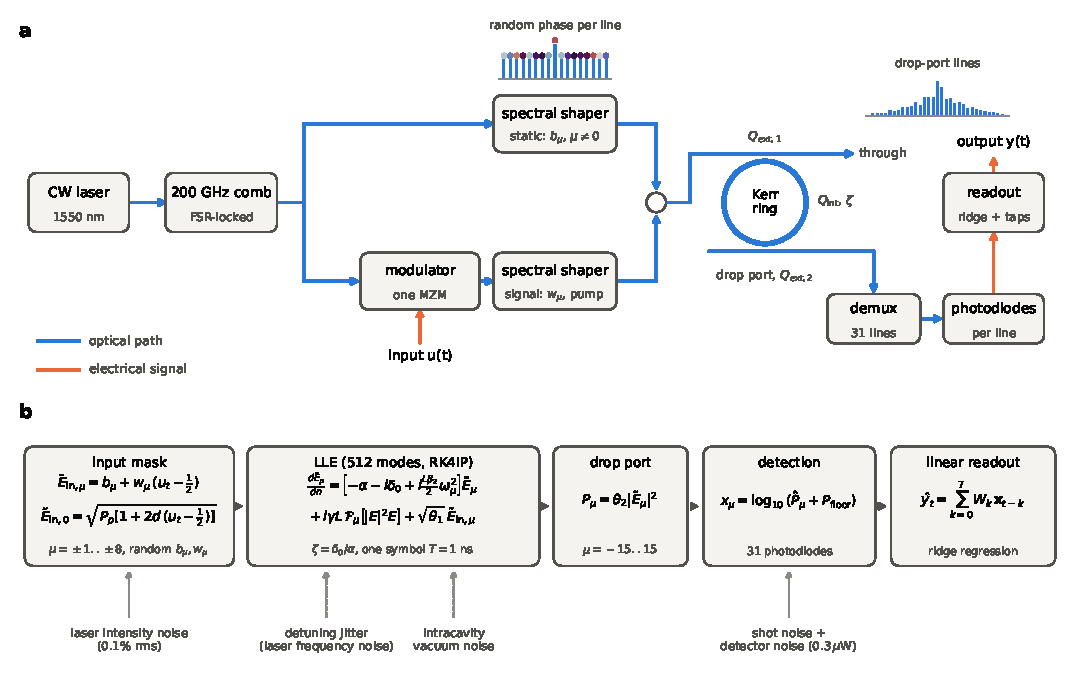
\includegraphics[width=\linewidth]{fig1_scheme}
\caption{Scheme and model.
(a) Optical layout. A $200~\mathrm{GHz}$ input comb locked to the resonator FSR is split in two: the static branch passes a
spectral phase shaper that writes the biases $b_\mu$; the other branch carries the signal $u(t)$ through one modulator and a
second shaper that writes the weights $w_\mu$. The recombined comb and the pump drive an add--drop Kerr ring (input coupling
$\Qone$, drop coupling $\Qtwo$, intrinsic $\Qint$, normalised detuning $\zeta$). The 31 drop-port lines are demultiplexed and
detected separately, and a ridge readout with delay taps combines them into the output $y(t)$. Insets: random phases of the input
lines (colour) and a sketch of the drop-port spectrum.
(b) Signal chain of the simulation model: input mask (Eq.~\eqref{eq:mask}), Lugiato--Lefever equation (Eq.~\eqref{eq:lle}),
drop-port power, logarithmic detection and linear readout; dashed arrows mark where the five noise sources enter
(Section~\ref{sec:noise-model}).}
\label{fig:scheme}
\end{figure}

The intracavity field is described by the mean-field Lugiato--Lefever equation (LLE)~\cite{lugiato1987,coen2013}.
With the round-trip number $n=t/t_R$ as slow time, the field amplitude $\tilde E_\mu$ of longitudinal mode $\mu$ (counted from the
pump), with angular frequency offset $\omega_\mu=2\pi\,\mathrm{FSR}\,\mu$, obeys
\begin{equation}
\frac{\mathrm d\tilde E_\mu}{\mathrm dn}
=\Big[-\alpha-i\delta_0+i\frac{L\beta_2}{2}\,\omega_\mu^{2}\Big]\tilde E_\mu
+i\gamma L\,\mathcal F_\mu\!\big[|E|^{2}E\big]
+\sqrt{\theta_1}\,\tilde E_{\mathrm{in},\mu}(u_t),
\label{eq:lle}
\end{equation}
where $E(\tau)$ is the intracavity field on the fast-time grid ($|E|^2$ in watts), $\mathcal F_\mu$ takes the $\mu$-th Fourier
component, $\theta_1$ and $\theta_2$ are the power coupling ratios of the two ports, $\alpha=(\alpha_i+\theta_1+\theta_2)/2$ is
the field loss per round trip (the half-linewidth), and $\delta_0$ is the pump detuning from resonance. We use the normalised
detuning $\zeta=\delta_0/\alpha$ (in half-linewidths), drawn in $[-1,4]$ for each operating point.
The loaded quality factor is $Q=\omega_0 t_R/(2\alpha)$, and the drop-port power of line $\mu$ is $P_\mu=\theta_2|\tilde E_\mu|^{2}$.

Equation~\eqref{eq:lle} is integrated with the fourth-order Runge--Kutta method in the interaction picture
(RK4IP)~\cite{hult2007}, which uses only fast Fourier transforms and pointwise operations, so gradients with respect to all device
parameters are available (Section~\ref{sec:gradient}).
By default we use 512 modes and 20 steps per $1~\mathrm{ns}$ symbol (about 200 round trips).
Results agree between 512 and 1024 modes (Appendix~\ref{app:checks}).

\subsection{Input encodings}\label{sec:encodings-def}

The input is a sequence of symbols $u_t\in[0,1]$, each held for $T=1~\mathrm{ns}$. We compare eight ways of feeding $u_t$ into the
resonator.

\paragraph{Spectral-phase input mask (this work).}
The input field consists of the pump ($\mu=0$) and eight input lines on each side ($\mu=\pm1,\dots,\pm8$):
\begin{equation}
\tilde E_{\mathrm{in},0}=\sqrt{P_p\,[1+2d\,(u_t-\tfrac12)]},\qquad
\tilde E_{\mathrm{in},\mu}=b_\mu+w_\mu\,(u_t-\tfrac12)\quad(\mu=\pm1,\dots,\pm8).
\label{eq:mask}
\end{equation}
The bias $b_\mu$ and modulation weight $w_\mu$ of every line are independent complex Gaussian numbers, i.e.\ random amplitudes and
random phases. They are scaled together so that the mean sideband power $\sum_\mu\big(|b_\mu|^{2}+|w_\mu|^{2}/12\big)$ is a fraction
$f_s$ of the total power $P$, and the pump power is $P_p=(1-f_s)P$.
The random parameters of an operating point are the total power $P$ ($10$ to $300~\mathrm{mW}$, log-uniform), $f_s\in[0.1,0.9]$,
the modulation depth $d\in[0.05,0.9]$, $\zeta$ and $\Qone$.
Experimentally this corresponds to splitting an input comb into a static branch (giving $b_\mu$) and a branch through one modulator
(giving $w_\mu$), each passing a programmable spectral shaper before recombination. The ablation of Section~\ref{sec:ablation}
shows that what matters is the randomness of the line phases, so the shapers need only set phases.

\paragraph{Single-pump encodings (literature schemes).}
A single CW pump whose power $P[1+d(u_t-\tfrac12)]$~\cite{shishavan2025}, detuning $\zeta+d(u_t-\tfrac12)$~\cite{cuevas2025} or
phase $\exp[i d(u_t-\tfrac12)]$~\cite{arabieh2026soliton} is modulated by the signal.
The power encoding uses $d\in[0.05,1]$; the detuning and phase encodings draw $d$ log-uniformly between $10^{-1.3}$ and $10^{0.5}$.
Each comes in two groups: the cavity starts from an empty field, or from a single soliton (the soliton groups draw $\zeta$ inside
the soliton existence range, $\Qone\in[10^{6.5},10^{7.2}]$ and $P\in[30,300]~\mathrm{mW}$).

\paragraph{Uniformly modulated comb.}
The same 16 input lines as the mask, but with equal amplitudes and equal phases, all modulated together by the same signal, which
corresponds to a modulated synchronous pulse train~\cite{arabieh2026pulse}.

All encodings use the same device, the same power and $Q$ ranges and the same readout, and draw the same number of random
operating points (Section~\ref{sec:protocol}).

\subsection{Readout}\label{sec:readout-def}

The central 31 lines of the drop port ($\mu=-15,\dots,15$) are demultiplexed and detected by separate photodiodes.
The readings are log-compressed, $x_\mu=\log_{10}(\hat P_\mu+P_\mathrm{floor})$, where $\hat P_\mu$ is the noisy reading and
$P_\mathrm{floor}$ the larger of the detector noise and $1~\mathrm{nW}$, so that dark lines do not dominate the regression after
the logarithm. Besides the 31 readings of the current symbol the readout sees those of the previous seven symbols (8 delay taps,
248 features; 12 taps for NARMA-10) and is a ridge regression on standardised features, with the regularisation chosen on the
validation part from $\{10^{-8},10^{-6},10^{-4},10^{-2},1\}$. Section~\ref{sec:memory} discusses the memory these taps provide.

\subsection{Noise model}\label{sec:noise-model}

``Realistic noise'' has three sources inside the device and two at detection:
\begin{itemize}
\item laser intensity noise: $0.1\%$ relative rms, one sample per symbol, shared by the pump and all input lines;
\item detuning jitter: the pump detuning from resonance fluctuates by $1\%$ of the half-linewidth (rms) per symbol, with a
      correlation time of one symbol; for white frequency noise this corresponds to a laser with an intrinsic linewidth of about
      $1.6~\mathrm{kHz}$ (Section~\ref{sec:laser} checks this against real laser frequency-noise spectra);
\item intracavity field noise at the vacuum level: half a photon per mode and loss channel;
\item shot noise, with each reading integrated over one symbol ($1~\mathrm{ns}$);
\item detector electronic noise of $0.3~\mu\mathrm{W}$ per line (rms, referred to optical power). For 1-GHz-class InGaAs PIN
      receivers the datasheet noise-equivalent power corresponds to $0.13$ to $0.63~\mu\mathrm{W}$ per line, so $0.3~\mu\mathrm{W}$
      is mid-range.
\end{itemize}
Amplified-spontaneous-emission beat noise and detector quantum efficiency are not modelled. Section~\ref{sec:noise} breaks down
the contribution of each source.

\subsection{Tasks and software baselines}\label{sec:tasks}

Three benchmark tasks:
(1) ten-step prediction of the Mackey--Glass series ($\tau=17$, $\beta=0.2$, $\gamma=0.1$, exponent 10, sampling interval 1);
(2) nonlinear channel equalisation~\cite{jaeger2004}: four-level symbols pass linear inter-symbol interference, a cubic
polynomial nonlinearity and additive noise at $28~\mathrm{dB}$ SNR, and the symbol sent two steps earlier is recovered from the
received signal (we report the symbol error rate besides the NMSE);
(3) NARMA-10, which needs a memory of about ten symbols.
Appendix~\ref{app:fibre} adds a realistic fibre-link task (28~GBd PAM-4 over 17~km of standard single-mode fibre, intensity
modulation and direct detection).

There are two software baselines. One is an echo state network (ESN)~\cite{jaeger2001} with 31 $\tanh$ nodes, matching the
resonator's readout dimension, whose readout sees the same delay taps and whose spectral radius and input scaling are chosen on the
validation part; Section~\ref{sec:software} adds ESNs of 100 to 1000 nodes and next-generation reservoir computing
(NG-RC)~\cite{gauthier2021}. The other is linear autoregression with up to 32 lagged inputs.
Under realistic noise the baselines receive input noise of $3\times10^{-3}$ rms, i.e.\ the laser intensity noise referred to the
input through a modulation depth of $0.33$; this convention strongly affects the comparison, and Section~\ref{sec:software} gives
the full sweep.

\subsection{Evaluation protocol}\label{sec:protocol}

Each series discards 300 warm-up symbols and then uses 1700 symbols, split 60/20/20 into training, validation and test parts (for
channel equalisation under realistic noise the test part is extended to 5000 symbols to resolve the symbol error rate).
Errors are normalised mean-square errors (NMSE). A physical device never sees the same noise twice, so the readout is always
trained on one run and tested on another run with independent noise (cross-run NMSE).

Operating points are chosen in two steps, so that a point that was merely lucky is not picked: for each encoding we draw 256
random operating points, run each once (a pair of runs) and keep the 16 best on validation error; these 16 are run on three new
pairs, and the one with the lowest mean validation error is chosen; we report its mean test error on six further new pairs.
Every setting is repeated on three independent series and the geometric mean is reported.
Choosing and reporting on a single noise realisation would be optimistic by 10 to 30\% (Appendix~\ref{app:checks}).
